%%%%%%%%%%%%%%%%%%%%%%%%%%%%%%%%%%%%%%%%%%%%%%%%%%%%%%%%%%%%%%%%%%%%%%%%%%%%%%%%%%%
%% Curtin Presentation Beamer Template                                           %%
%% Adapted from UFC template by
%% author: Maurício Moreira Neto - Doctoral student in Computer Science (MDCC)   %%
%%%%%%%%%%%%%%%%%%%%%%%%%%%%%%%%%%%%%%%%%%%%%%%%%%%%%%%%%%%%%%%%%%%%%%%%%%%%%%%%%%%

\documentclass{libs/curtin_format}
\usepackage{subcaption}
% Inserting the preamble file with the packages
%%%%%%%%%%%%%%%%%%%%%%%%%%%%%%%%%%%%%%%%%%%%%%%%%%%%%%%%%%%%%%%%%%%%%
%% This file contains the packages that can be used in the beamer. %%
%%%%%%%%%%%%%%%%%%%%%%%%%%%%%%%%%%%%%%%%%%%%%%%%%%%%%%%%%%%%%%%%%%%%%
% Package to fonts family
\usepackage[T1]{fontenc}
% Package to accentuation
\usepackage[utf8]{inputenc}
% Package to Portuguese language
%\usepackage[brazil]{babel}

%just in case eps figures are available instead - automatically converted to PDF
\usepackage{epstopdf}

% Package to Figures
\usepackage{graphicx}
% Package to the colors
\usepackage{color}
% Package to the colors
\usepackage{xcolor}
% Packages to math symbols and expressions
\usepackage{amsfonts, amssymb, amsmath}
% Package to multiple lines and columns in table
\usepackage{multirow, array} 
% Package to create pseudo-code
% For more detail of this package: http://linorg.usp.br/CTAN/macros/latex/contrib/algorithm2e/doc/algorithm2e.pdf
\usepackage{algorithm2e}
% Package to insert code
\usepackage{listings} 
\usepackage{keyval}
% Package to justify text
\usepackage[document]{ragged2e}
% Package to manage the bibliography
% \usepackage[backend=biber, style=numeric, sorting=none]{biblatex}
% Package to facilities quotations
\usepackage{csquotes}
% Package to use multicols
\usepackage{multicol}


% Inserting the references file
\bibliography{references-crackseg.bib}
%\usepackage[style=author,backend=bibtex]{biblatex}
%\addbibresource{references.bib}

% \begin{figure}
%         \centering        
%         \includegraphics[width=2.00cm,height=1.00cm]{figs/ICONIP2021_logo.eps}
%         %\caption{Example of semantic segmentation}        
%         \label{fig:logo}
% 	\end{figure}	
% \vspace{-0.4cm}

% Title
\title[SC-CrackSeg]{\huge\textbf{SC-CrackSeg: A Real-time Shared Feature Pyramid
Network for Crack Detection and Segmentation}}
% Subtitle
%\subtitle{ICONIP 2021}

% Author of the presentation
\author{T. Singha, M. Bergemann, D.S. Pham, and A. Krishna}
% Institute's Name
\institute[Curtin]{
    % email for contact
    \normalsize{\email{}}
    \newline
    % Department Name
    \department{School of EECMS}
    %\newline
    % university name
    \curtin
}
% date of the presentation
\date{}


%%%%%%%%%%%%%%%%%%%%%%%%%%%%%%%%%%%%%%%%%%%%%%%%%%%%%%%%%%%%%%%%%%%%%%%%%%%%%%%%%%
%% Start Document of the Presentation                                           %%               
%%%%%%%%%%%%%%%%%%%%%%%%%%%%%%%%%%%%%%%%%%%%%%%%%%%%%%%%%%%%%%%%%%%%%%%%%%%%%%%%%%
\begin{document}
% insert the code style
%%%%%%%%%%%%%%%%%%%%%%%%%%%%%%%%%%%%%%%%%%%%%%%%%%%%%%%%%%%%%%%%%%%%%%%%%%%%%%%%%%%
%% This file contains the style of the codes show in slides.                     %%
%% The package used is listings, but it possible to used others.                 %%
%%%%%%%%%%%%%%%%%%%%%%%%%%%%%%%%%%%%%%%%%%%%%%%%%%%%%%%%%%%%%%%%%%%%%%%%%%%%%%%%%%%

% color used in the code style
\definecolor{codegreen}{rgb}{0,0.6,0}
\definecolor{codegray}{rgb}{0.5,0.5,0.5}
\definecolor{codepurple}{rgb}{0.58,0,0.82}
\definecolor{codebackground}{rgb}{0.95,0.95,0.92}

% style of the code!
\lstdefinestyle{codestyle}{
    backgroundcolor=\color{codebackground},   
    commentstyle=\color{codegreen},
    keywordstyle=\color{magenta},
    numberstyle=\tiny\color{codegray},
    stringstyle=\color{codepurple},
    basicstyle=\ttfamily\footnotesize,
    frame=single,
    breakatwhitespace=false,         
    breaklines=true,                 
    captionpos=b,                    
    keepspaces=true,                 
    numbers=left,                    
    numbersep=5pt,                  
    showspaces=false,                
    showstringspaces=false,
    showtabs=false,                  
    tabsize=2,
    title=\lstname 
}

\lstset{style=codestyle}


%% ---------------------------------------------------------------------------
% First frame (with tile, subtitle, ...)
\begin{frame}{}	

    \maketitle
	\vspace{-0.4cm}
	\begin{figure}
        \centering        
        \includegraphics[width=2.00cm,height=0.9cm]{figs/DICTA_2022_logo.eps}
        %\caption{Example of semantic segmentation}        
        \label{fig:logo}
	\end{figure}	

\end{frame}

%% ---------------------------------------------------------------------------
% Second frame
\begin{frame}{Table of Contents}
    %\begin{multicols}{2}
        \tableofcontents
    %\end{multicols}
\end{frame}

%% ---------------------------------------------------------------------------
% This presentation is separated by sections and subsections
\section{Overview of key contributions}
\begin{frame}{Overview of key contributions}
Our key contributions are:
	\begin{itemize}
		\item Introduce a new efficient shared branch semantic segmentation network designed specifically for crack segmentation
		\item Evaluated a new challenging crack dataset consisting of multiple other datasets merged together
		\item Evaluated performance of our model and other models on new dataset, indicating our model achieves state of the art performance at a low number of FLOPs \& parameters
	\end{itemize}
\end{frame}

\section{Background}
\begin{frame}{Overview of of crack segmentation}
\vspace{0.1cm}
    \begin{itemize}
        \item \textbf{Semantic Segmentation}- The pixel-wise classification of an image
        \item Important for structural damage detection - crack shape/size is valuable information
        \item Efficiency is sought after due to large scale of structural damage detection \cite{kerle_uav-based_2020} \cite{kang_autonomous_2018}
    \end{itemize}

    \begin{figure}
    \centering
    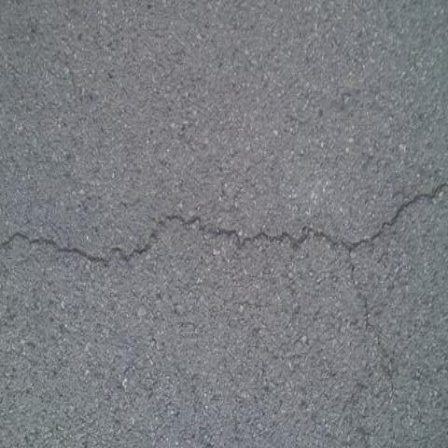
\includegraphics[width=0.8\linewidth]{figs-crackseg/dataset_CFD_029.eps}
    \caption{Crack dataset sam-le}
    \label{fig:crack-percentages-sub1}
    \end{subfigure}%
    \begin{subfigure}{.3\textwidth}
        \centering
        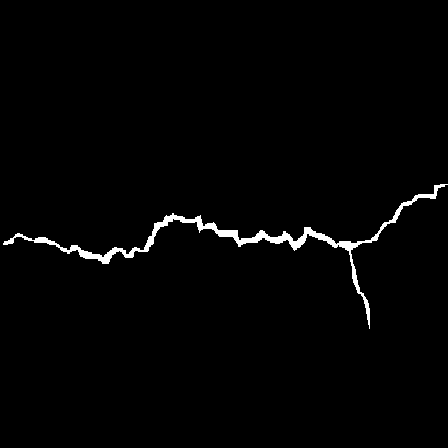
\includegraphics[width=0.8\linewidth]{figs-crackseg/dataset_CFD_029_label.eps}
        \caption{Crack label}
        \label{fig:crack-percentages-sub2}
    \end{subfigure}
    \caption{Crack image and corresponding segmentation mask from the CFD dataset \cite{shi2016automatic}.}
    \label{fig:crack-percentages}
\end{figure}

\end{frame}

\begin{frame}{Our motivation}
\vspace{0.1cm}
    Several key issues in crack segmentation:
    \begin{itemize}
        \item Cracks are thin and fine - must extract highly dense features
        \item Crack segmentation is imbalanced - $<1:20$ ratio of crack to background
        \item Existing approaches (DeepCrack \cite{liu2019deepcrack}, FPHBN \cite{yang2019feature}, MR-CrackNet \cite{nayyeri2021multi}) tackle these, but models/datasets often unavailable
    \end{itemize}
    Our realisation - maintaining global perspective while focusing on shallow features is achieved by \textbf{multi-branch networks} (BiSeNet \cite{yu2018bisenet}, ContextNet, \cite{poudel2018contextnet}, SCMNet)\cite{singha2021scmnet})
    % \vspace{-0.1cm} % vertical space
    \begin{figure}
        \centering
        \includegraphics[width=\linewidth,height=2.50cm]{figs-crackseg/contextnet.png}
        \caption{Architecture of ContextNet \cite{poudel2018contextnet}.}
        \label{fig:farme2}
    \end{figure}
\end{frame}

\begin{frame}{SCMNet}
\vspace{0.1cm}
    \begin{itemize}
        \item We use SCMNet \cite{singha2021scmnet} as our base model
        \item Apply modifications for crack segmentation, streamline, and improve efficiency
    \end{itemize}
    % \vspace{-0.1cm} % vertical space
    \begin{figure}
        \centering
        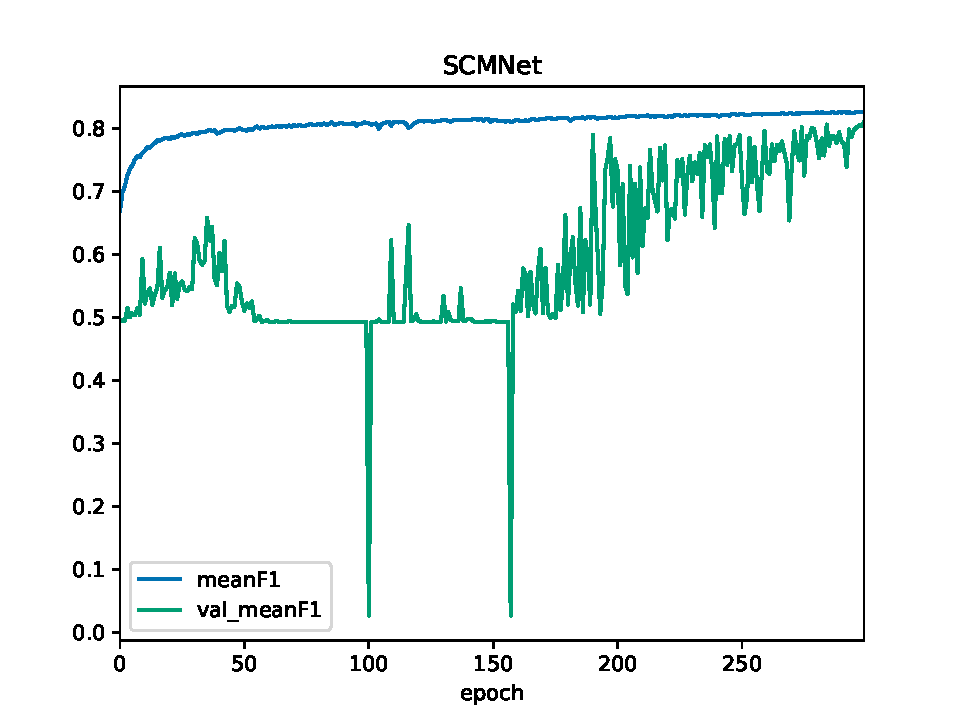
\includegraphics[width=\linewidth,height=2.50cm]{figs-crackseg/scmnet.eps}
        \caption{Architecture of SCMNet \cite{singha2021scmnet}.}
        \label{fig:farme2}
    \end{figure}
\end{frame}
 % --------------------------------------------------------------------------- %
\section{Model Architecture}

\begin{frame}{Complete Pipeline}
\begin{itemize}
        \item Shared encoder (periodic information sharing between branches)
        \item Single-input encoder
        \item Simplified decoder
    \end{itemize}
    %\vspace{0.1cm} % vertical space
   \begin{figure}
        \centering        
        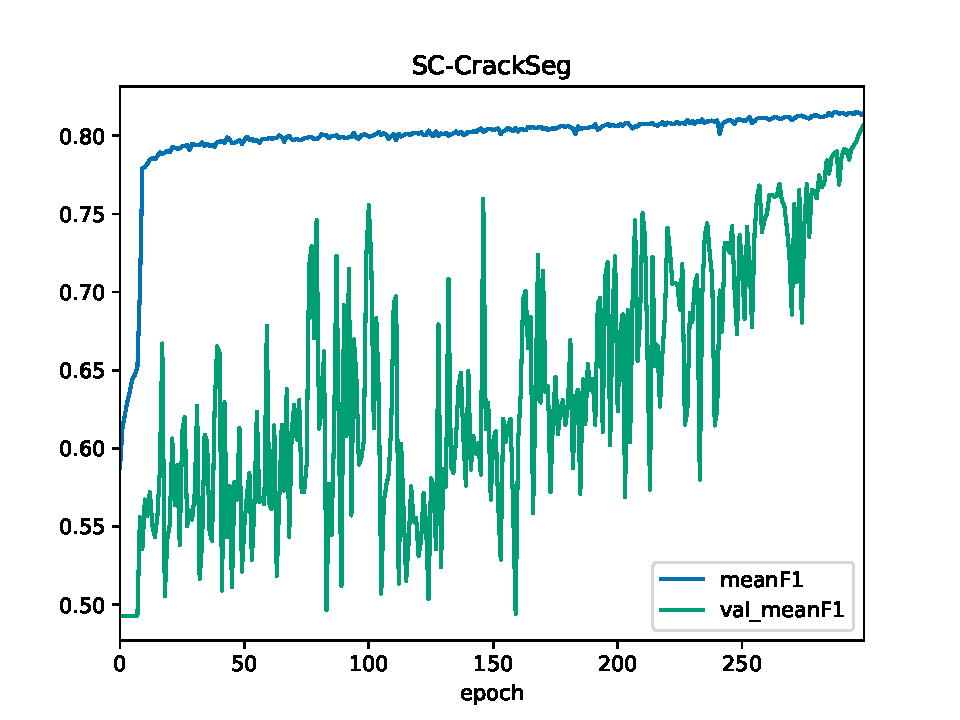
\includegraphics[width=\linewidth,height=3.50cm]{figs-crackseg/sc-crackseg.eps}
        \caption{Complete architecture of SC-CrackSeg}        
        \label{fig:pipeline}
    \end{figure}
\end{frame}

\begin{frame}{Shared Context Refinement Module}
\begin{itemize}
        \item Replaces SCMNet's CMM
        \item Performs multi-scale extraction (similar to atrous spatial pyramid pooling \cite{chen2017deeplab})
    \end{itemize}
    %\vspace{0.1cm} % vertical space
   \begin{figure}
        \centering        
        \includegraphics[width=\linewidth,height=3.50cm]{figs-crackseg/shared-crm.eps}
        \caption{Architecture of the Shared Context Refinement Module}        
        \label{fig:pipeline}
    \end{figure}
\end{frame}

\begin{frame}{Decoder Design}
\begin{itemize}
        \item Semantic Aggregation (SA) Module extracts multi-level features
        \item Depthwise Separable convolutions + + classification + $8 \times$ upsample
    \end{itemize}
    %\vspace{0.1cm} % vertical space
   \begin{figure}
        \centering        
        \includegraphics[width=\linewidth,height=3.50cm]{figs-crackseg/sam.eps}
        \caption{Architecture of the Semantic Aggregation Module}
        \label{fig:pipeline}
    \end{figure}
\end{frame}

% ---------------------------------------------------------------------------


\section{Evaluation}
\begin{frame}{Dataset}
\begin{itemize}
        \item Used combination of 12 existing crack segmentation datasets
        \item Wide variety in crack types
        \item 11,200 $448 \times 448$ images
    \end{itemize}
    %\vspace{0.1cm} % vertical space
   \begin{figure}
        \centering        
        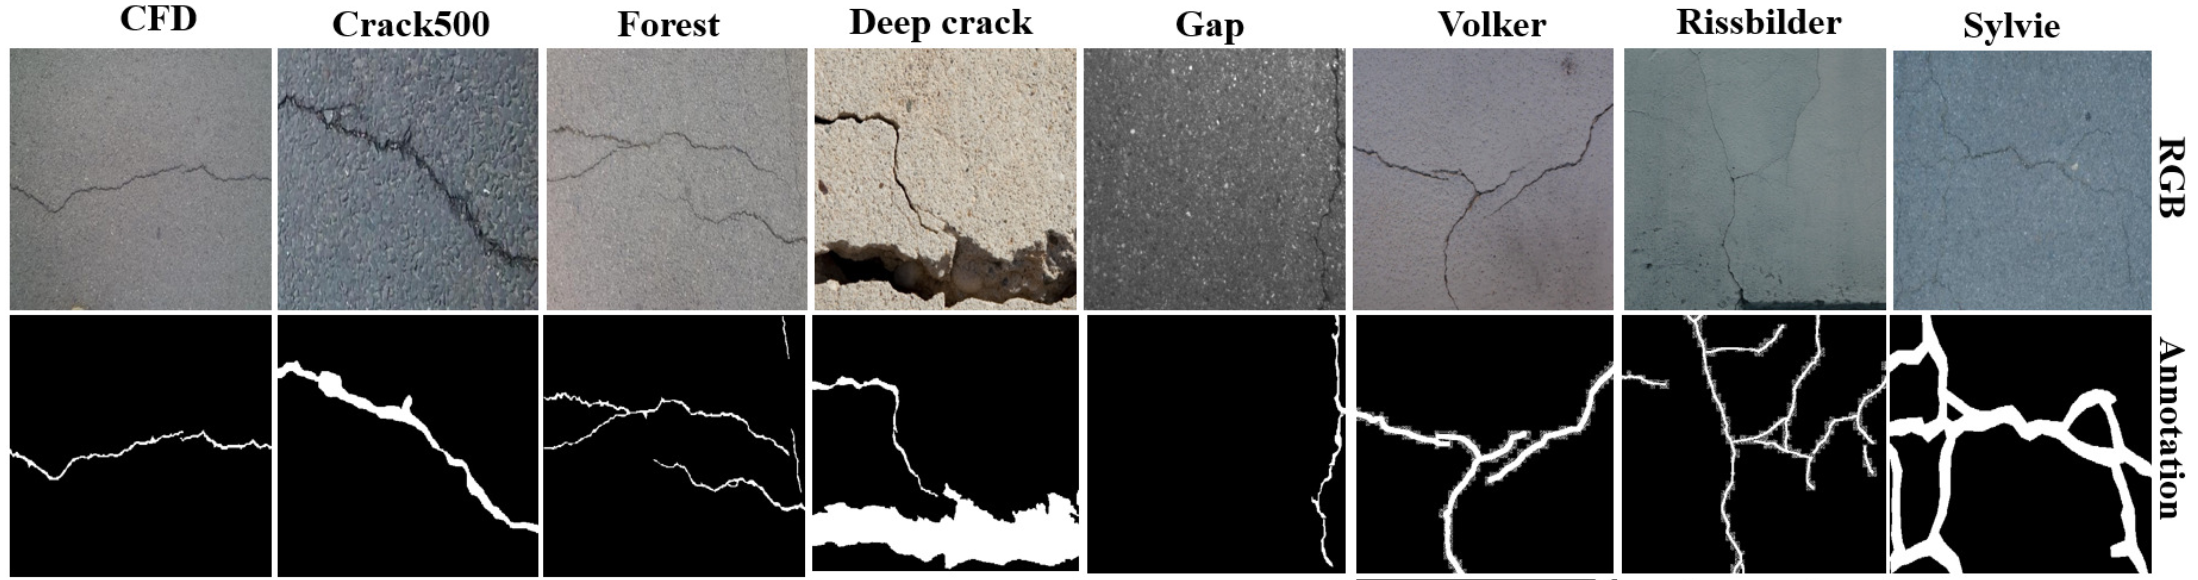
\includegraphics[width=\linewidth,height=3.50cm]{figs-crackseg/crack-dataset.png}
        \caption{Samples from the merged crack dataset}
        \label{Fig:annotation}
    \end{figure}
\end{frame}

\begin{frame}{Dataset issues}
\begin{itemize}
        \item Compression artefacts present in dataset labels
        \item Ignored all artefacts
    \end{itemize}
    %\vspace{0.1cm} % vertical space
   \begin{figure}
        \centering        
        \includegraphics[width=\linewidth,height=3.50cm]{figs-crackseg/dataset-processing.eps}
        \caption{Processing of dataset. (a) RGB input, (b) Actual annotation, (c) Displaying noisy pixel, (d) Processed annotation}
        \label{Fig:annotation}
    \end{figure}
\end{frame}

\begin{frame}{Ablation study}
\begin{table}[htbp]
    \caption{Result of ablation study}\label{tab3}
        \centering
        \begin{tabular}{|c|c|c|c|c|c|c|c|}
        \hline
        {\begin{tabular}{@{}c@{}}No. of\\input in the\\backbone\end{tabular}} & {CMM} & {CRM} & {Decoder} & {mF1(\%)} & {P(\%)} & {R(\%)}\\
        \hline
        {Two} & {\checkmark} & {-} & {-} & {73.0} & {75.6} & {70.5}\\
        \hline
        {One} & {\checkmark} & {-} & {-} & {75.9} & {78.3} & {73.6}\\
        \hline
        {One} & {} & {\checkmark} & {-} & {82.2} & {84.6} & {80.0}\\
        \hline
        {One} & {} & {\checkmark} & {\checkmark} & {85.3} & {88.6} & {82.3}\\
        \hline
        \multicolumn{7}{l}{}
        \end{tabular}
    \end{table}
\end{frame}

\begin{frame}{Quantitative Results}
    \resizebox{\columnwidth}{!}{%

    \begin{table*}[htbp]
    \caption{Performance evaluation of different models on crack test set}\label{tab5}
        \centering
        \begin{tabular}{|c|c|c|c|c|c|c|c|c|c|c|c|c|c|}
        \hline
        & & \multicolumn{3}{|c|}{\textbf{IoU}} & \multicolumn{3}{|c|}{\textbf{F1 score}} & \multicolumn{3}{|c|}{\textbf{Precision}} & \multicolumn{3}{|c|}{\textbf{Recall}}\\
        \hline
        {Model} & {Accuracy} & {BG} & {Crack} & {mIoU} & {BG} & {Crack} & {mF1} & {BG} & {Crack} & {aP} & {BG} & {Crack} & {aR}\\
        \hline
        {DeepLab \cite{chen2018encoder}} & {98.43} & {98.50} & {52.28} & {75.39} & {99.24} & {68.66} & {83.95} & {98.97} & {79.25} & {89.11} & {99.52} & {60.57} & {80.05}\\
        \hline
        {Unet \cite{}} & {98.18} & {98.2} & {48.97} & {73.58} & {99.09} & {65.74} & {82.42} & {98.96} & {70.62} & {84.79} & {99.23} & {61.49} & {80.20}\\
        \hline
        {SegNet\cite{chen_pavement_2020}} & {98.27} & {98.30} & {52.17} & {75.23} & {99.14} & {68.57} & {83.85} & {99.09} & {71.15} & {85.12} & {99.19} & {66.17} & {82.63}\\
        \hline
        {DeepCrack\cite{liu2019deepcrack}} & \textbf{98.52} & {98.57} & {55.89} & \textbf{77.23} & {99.28} & {71.70} & \textbf{85.49} & {99.13} & {77.95} & {84.54} & {99.44} & {66.38} & \textbf{82.91}\\
        \hline
        {MR-CrackNet\cite{nayyeri2021multi}} & {97.88} & {97.19} & {47.69} & {72.80} & {98.95} & {64.58} & {81.76} & {99.11} & {62.59} & {80.85} & {98.79} & {66.71} & {82.70}\\
        \hline
        {SCMNet\cite{singha2021scmnet}} & {98.39} & {98.41} & {51.33} & {74.87} & {99.20} & {67.84} & {83.52} & {98.91} & {77.51} & {88.21} & {99.48} & {60.32} & {79.30}\\
        \hline
        {SC-CrackSeg} & \textbf{98.52} & {98.52} & {55.55} & {77.04} & {99.25} & {71.43} & {85.34} & {99.05} & {78.14} & \textbf{88.59} & {99.46} & {65.78} & {82.32}\\
        \hline
        \multicolumn{11}{l}{}
        \end{tabular}
    \end{table*}
    }
\end{frame}

\begin{frame}{Qualitative Results}
   \begin{figure}
        \centering        
        \includegraphics[width=\linewidth]{figs-crackseg/qualitative-results.eps}
        \caption{Output of different models on test sample}
        \label{fig:pipeline}
    \end{figure}
\end{frame}

\begin{frame}{Qualitative Results}
   \begin{figure}
        \centering        
        \includegraphics[width=\linewidth]{figs-crackseg/varied-results.eps}
        \caption{Qulaitative results from different samples in test set}
        \label{fig:pipeline}
    \end{figure}
\end{frame}


\begin{frame}{Model efficiency}
    \resizebox{\columnwidth}{!}{%
    \begin{table*}
    \caption{Efficiency analysis}\label{tab6}
        \centering
        \begin{tabular}{|c|c|c|c|c|c|c|c|c|c|}
        \hline
        {}& {} & {} & \multicolumn{5}{|c|}{\textbf{FPS of different types of model}} &  {} & {}\\
        \hline
        {Model} & {Param.(M)} & {GFLOPs} & {Keras} & {TF} & {TF-TRT32} & {TF-TRT16} & {TRT-INT8} & {\begin{tabular}{@{}c@{}}Training\\time(s)\end{tabular}} &
        {\begin{tabular}{@{}c@{}}Model \\size (MB)\end{tabular}}\\
        \hline
        {DeepLab} & {41.0} & {78.8} & {20} &  {21} & {32} & {48} &  {82} & {415} & {158}\\
        \hline
        {Unet} & {31.0} & {1740.0} & {31} &  {30} & {39} & {39} &  {50} & {348} & {355}\\
        \hline
        {SegNet} & {29.4} & {245.0} & {32} &  {32} & {44} & {45} &  {56} & {316} & {225}\\
        \hline
        {DeepCrack} & {14.7} & {123.0} & {33} &  {33} & {48} & {50} &  {65} & {257} & {112}\\
        \hline
        {MR-CrackNet} & {17.7} & {331} & {14} &  {14} & {25} & {28} &  {45} & {1013} & {203}\\
        %\hline
        %{MR-CrackNet} & {17.7} & {331} & {} &  {} & {} & {} &  {} & {} & {}\\
        \hline
        {SCMNet} & \textbf{1.2} & {3.3} & {61} &  {67} & {111} & {111} &  {114} & {182} & {10.7}\\
        \hline
        {SC-CrackSeg} & {1.24} & \textbf{2.8} & \textbf{70} &  \textbf{78} & \textbf{216} & \textbf{216} &  \textbf{220} & \textbf{93} & \textbf{10.8}\\
        \hline
        \multicolumn{10}{l}{}
        \end{tabular}
    \end{table*}
    }
\end{frame}

% ---------------------------------------------------------------------------
%% ---------------------------------------------------------------------

%% ---------------------------------------------------------------------------
% Reference frames
\begin{frame}[t,allowframebreaks]
    \frametitle{References}
    \printbibliography
\end{frame}

%% ---------------------------------------------------------------------------
% Final frame
\begin{frame}{}
    \centering
    \huge{\textbf{\example{Thank you!}}}
    
    \vspace{1cm}
    
    \Large{\textbf{Contact:}}
    \newline
    \vspace*{0.5cm}
    \large{\email{tanmay.singha@postgrad.curtin.edu.au}}
    \large{\email{moritz.bergemann@student.curtin.edu.au}}
\end{frame}

\end{document}